\documentclass[12pt,a4paper]{article}
\usepackage[utf8]{inputenc}
\usepackage{dsfont} 
\usepackage[polish]{babel}
\usepackage{amsmath}
\usepackage{graphicx}
\usepackage[top=1in, bottom=1.5in, left=1.25in, right=1.25in]{geometry}
\usepackage[utf8]{inputenc}
\usepackage[polish]{babel}
\usepackage{subfig}
\usepackage{multirow}
\usepackage{multicol}
\graphicspath{{Imagens/}}
\usepackage{xcolor,colortbl}
\usepackage{float}
\usepackage{polski}
\usepackage[utf8]{inputenc}
\newcommand \comment[1]{\textbf{\textcolor{red}{#1}}}

%\usepackage{float}
\usepackage{fancyhdr} % Required for custom headers
\usepackage{lastpage} % Required to determine the last page for the footer
\usepackage{extramarks} % Required for headers and footers
\usepackage{indentfirst}
\usepackage{placeins}
\usepackage{scalefnt}
\usepackage{xcolor,listings}
\usepackage{textcomp}
\usepackage{color}
\usepackage{verbatim}
\usepackage{framed}

\definecolor{codegreen}{rgb}{0,0.6,0}
\definecolor{codegray}{rgb}{0.5,0.5,0.5}
\definecolor{codepurple}{HTML}{C42043}
\definecolor{backcolour}{HTML}{F2F2F2}
\definecolor{bookColor}{cmyk}{0,0,0,0.90}  
\color{bookColor}

\lstset{upquote=true}

\lstdefinestyle{mystyle}{
	backgroundcolor=\color{backcolour},   
	commentstyle=\color{codegreen},
	keywordstyle=\color{codepurple},
	numberstyle=\numberstyle,
	stringstyle=\color{codepurple},
	basicstyle=\footnotesize\ttfamily,
	breakatwhitespace=false,
	breaklines=true,
	captionpos=b,
	keepspaces=true,
	numbers=left,
	numbersep=10pt,
	showspaces=false,
	showstringspaces=false,
	showtabs=false,
}
\lstset{style=mystyle}

\newcommand\numberstyle[1]{%
	\footnotesize
	\color{codegray}%
	\ttfamily
	\ifnum#1<10 0\fi#1 |%
}

\definecolor{shadecolor}{HTML}{F2F2F2}

\newenvironment{sqltable}%
{\snugshade\verbatim}%
{\endverbatim\endsnugshade}

% Margins
\addtolength{\footskip}{0cm}
\addtolength{\textwidth}{1.4cm}
\addtolength{\oddsidemargin}{-.7cm}

\addtolength{\textheight}{1.6cm}
%\addtolength{\topmargin}{-2cm}

% paragrafo
\addtolength{\parskip}{.2cm}

% Set up the header and footer
\pagestyle{fancy}
\rhead{\hmwkAuthorName} % Top left header
\lhead{\hmwkClass: \hmwkTitle} % Top center header
\rhead{\firstxmark} % Top right header
\lfoot{Gracjan Kościński} % Bottom left footer
\cfoot{} % Bottom center footer
\rfoot{} % Bottom right footer
\renewcommand{\headrulewidth}{1pt}
\renewcommand{\footrulewidth}{1pt}

    
\newcommand{\hmwkTitle}{Aplikacja do zarządzania zadaniami} % Tytuł projektu
\newcommand{\hmwkDueDate}{\today} % Data 
\newcommand{\hmwkClass}{Technologie chmurowe} % Nazwa przedmiotu
\newcommand{\hmwkAuthorName}{Gracjan Kościński} % Imię i nazwisko

% trabalho 
\begin{document}
% capa
\begin{titlepage}
    \vfill
	\begin{center}
	\hspace*{-1cm}
	\vspace*{0.5cm}
    
\includegraphics[scale=0.55]{imagens/loga.png}\\
	\textbf{Uniwersytet Gdański \\ [0.05cm]Wydział Matematyki, Fizyki i Informatyki \\ [0.05cm] Instytut Informatyki}

	\vspace{0.6cm}
	\vspace{4cm}
	{\huge \textbf{\hmwkTitle}}\vspace{8mm}
	
	{\large \textbf{\hmwkAuthorName}}\\[3cm]
	
		\hspace{.45\textwidth} %posiciona a minipage
	   \begin{minipage}{.5\textwidth}
	   Projekt z przedmiotu technologie chmurowe na kierunku informatyka profil praktyczny na Uniwersytecie Gdańskim.\\[0.1cm]
	  \end{minipage}
	  \vfill
	%\vspace{2cm}
	
	\textbf{Gdańsk}
	
	\textbf{\hmwkDueDate}
	\end{center}
	
\end{titlepage}

\newpage
\setcounter{secnumdepth}{5}
\tableofcontents
\newpage

\section{Opis projektu}
\label{sec:Project}
W dzisiejszym dynamicznie zmieniającym się świecie, firmy coraz częściej stają przed wyzwaniem skutecznego zarządzania swoimi aplikacjami i danymi. Firma ABC, napotkała problem zarządzania zadaniami przydzielanymi pracownikom oraz konieczności utrzymania wysokiej wydajności aplikacji przy jednoczesnym zapewnieniu skalowalności i bezpieczeństwa. Projekt ten ma na celu stworzenie rozwiązania opartego na Kubernetes, które integruje frontend, backend, bazę danych oraz system zarządzania tożsamościami Keycloak, aby sprostać tym wymaganiom.
\subsection{Opis architektury}
\label{sec:introduction}
Architektura aplikacji jest oparta na Kubernetes, który zapewnia skalowalność,\\ automatyzację zarządzania kontenerami oraz wysoką dostępność. Klaster Kubernetes \\ zarządza wdrożeniami, skalowaniem oraz konfiguracją wszystkich komponentów aplikacji.

\textbf{Komponenty architektury:}
\begin{itemize}
    \item \textbf{Kubernetes Cluster} Podstawowy element architektury, odpowiedzialny za \\zarządzanie kontenerami. Składa się z węzłów master i worker, które współpracują, aby zarządzać obciążeniem aplikacji.
    \item \textbf{Frontend} Aplikacja oparta na Next.js, uruchamiana w kontenerze. Obsługuje \\interfejs użytkownika i komunikuje się z backendem.
    \item \textbf{Backend} Serwis w python, który obsługuje logikę biznesową i komunikację z bazą danych oraz systemem Keycloak.
    \item \textbf{Baza danych (PostgreSQL)} Przechowuje dane aplikacji. Uruchamiana jako osobny kontener, z wykorzystaniem Persistent Volume Claim (PVC) do zapewnienia trwałości danych.
    \item \textbf{Keycloak} System zarządzania tożsamościami i uwierzytelnianiem.\\ Zapewnia bezpieczne logowanie użytkowników oraz zarządzanie sesjami.
\end{itemize}

\subsection{Opis infrastruktury}
\label{sec:Users}

Aplikacja działa w środowisku chmurowym, wykorzystując platformę Kubernetes do zarządzania kontenerami. Infrastruktura składa się z następujących elementów:
\begin{itemize}
    \item \textbf{Platforma chmurowa} Kubernetes
    \item \textbf{Sieć} Wykorzystanie ClusterIP do wewnętrznej komunikacji między usługami, oraz NodePort/LoadBalancer do eksponowania usług na zewnątrz klastra.
    \item \textbf{Pamięć masowa} Persistent Volume Claims (PVC) do zarządzania trwałością danych w bazie PostgreSQL.
\end{itemize}
\subsection{Opis komponentów aplikacji}
\label{sec:FunctionalConditions}

Każdy komponent aplikacji jest uruchamiany jako osobny kontener w klastrze Kubernetes.
\begin{enumerate}
    \item \textbf{Frontend}
    \begin{itemize}
        \item \textbf{Implementacja} Next.js
        \item \textbf{Wdrożenie} Kontener Docker
        \item \textbf{Konfiguracja} Zmienne środowiskowe zarządzane przez ConfigMap
        \item \textbf{Zarządzanie} Automatyczne skalowanie
    \end{itemize}
    \item \textbf{Backend}
    \begin{itemize}
        \item \textbf{Implementacja} Python Flask
        \item \textbf{Wdrożenie} Kontener Docker
        \item \textbf{Konfiguracja}  Zmienne środowiskowe zarządzane przez ConfigMap
        \item \textbf{Zarządzanie} Automatyczne skalowanie
    \end{itemize}
    \item \textbf{PostgreSQL}
    \begin{itemize}
        \item \textbf{Implementacja} PostgreSQL
        \item \textbf{Wdrożenie} Kontener Docker
        \item \textbf{Konfiguracja} Zmienne środowiskowe zarządzane przez ConfigMap i Secret
        \item \textbf{Zarządzanie} Persistent Volume Claim (PVC) zapewniające trwałość danych
    \end{itemize}
    \item \textbf{Keycloak}
    \begin{itemize}
        \item \textbf{Implementacja} Keycloak
        \item \textbf{Wdrożenie} Kontener Docker
        \item \textbf{Konfiguracja} Zmienne środowiskowe zarządzane przez ConfigMap
        \item \textbf{Zarządzanie} Automatyczne skalowanie
    \end{itemize}
\end{enumerate}
\newpage
\subsection{Konfiguracja i zarządzanie}
\label{sec:NonFunctionalConditions}

Konfiguracja i zarządzanie aplikacją na poziomie klastra Kubernetes obejmuje:
\begin{itemize}
    \item \textbf{ConfigMap} Przechowywanie konfiguracji niezawierającej wrażliwych danych
    \item \textbf{Secrets} Przechowywanie wrażliwych danych, takich jak hasła i klucze API.
\end{itemize}

Zarządzanie aplikacją w klastrze Kubernetes odbywa się również za pomocą Kubernetes Dashboard, które jest intuicyjnym interfejsem graficznym umożliwiającym monitorowanie i zarządzanie zasobami Kubernetes. Dashboard pozwala użytkownikom na przeglądanie stanu klastra, wdrożonych aplikacji oraz dostępnych zasobów w sposób bardziej przyjazny niż korzystanie wyłącznie z interfejsu wiersza poleceń kubectl.

Dzięki Kubernetes Dashboard, użytkownicy mogą:
\begin{itemize}
\item Monitorować ogólny stan klastra, w tym sprawność węzłów oraz działających na nich podów.
\item Przeglądać szczegółowe informacje o wdrożonych aplikacjach, takich jak liczba replik, użycie zasobów, stan poszczególnych podów oraz logi aplikacji.
\item Zarządzać konfiguracją aplikacji, w tym modyfikować ConfigMap i Secrets bezpośrednio z poziomu interfejsu graficznego.
\item Tworzyć i usuwać zasoby, takie jak pody, usługi, deploymenty oraz inne obiekty Kubernetes.
\item Sprawdzać aktualne użycie zasobów (CPU, pamięć) przez poszczególne komponenty aplikacji, co umożliwia optymalizację wykorzystania zasobów i szybszą identyfikację potencjalnych problemów wydajnościowych.
\end{itemize}

Aby dane dotyczące użycia zasobów były dostępne w Dashboard, konieczna jest instalacja i prawidłowa konfiguracja Metrics Server. Metrics Server jest kluczowym komponentem w ekosystemie Kubernetes, który zbiera metryki dotyczące użycia zasobów (CPU i pamięci) z kubeletów na węzłach i udostępnia je innym komponentom, takim jak Horizontal Pod Autoscaler, który automatycznie skalibruje liczbę replik podów w odpowiedzi na zmieniające się obciążenie aplikacji.

Metrics Server jest lekki i zaprojektowany do pracy w klastrach produkcyjnych. Gdy jest zainstalowany, Dashboard może wyświetlać aktualne metryki, co znacznie ułatwia monitorowanie wydajności i zdrowia aplikacji oraz szybką reakcję na wszelkie problemy. Dzięki temu administratorzy i deweloperzy mają lepszy wgląd w działanie swoich aplikacji i mogą skuteczniej zarządzać zasobami klastra.

Podsumowując, Kubernetes Dashboard w połączeniu z Metrics Server stanowi potężne narzędzie do zarządzania i monitorowania aplikacji w klastrze Kubernetes, zapewniając łatwość obsługi oraz głęboki wgląd w wydajność i stan działania wdrożonych aplikacji.
\newpage
\subsection{Zarządzanie błędami}
\label{sec:ERD} 
Zarządzanie błędami w aplikacjach opartych na Kubernetes jest kluczowym elementem zapewnienia stabilności, niezawodności i wysokiej dostępności systemu. Skuteczne zarządzanie błędami obejmuje zarówno prewencję, jak i odpowiednie reakcje na występujące awarie, mające na celu szybkie przywrócenie działania aplikacji oraz minimalizację wpływu na użytkowników końcowych.
\textbf{Sposoby zarządzania błędami}
\begin{itemize}
    \item \textbf{Monitorowanie} Monitorowanie stanu aplikacji odgrywa kluczową rolę w wczesnym wykrywaniu potencjalnych problemów i błędów.
    \item \textbf{Automatyczne skalowanie i replikacja} W przypadku nagłego wzrostu obciążenia lub awarii jednego z podów, Kubernetes umożliwia automatyczne skalowanie i replikację podów za pomocą Horizontal Pod Autoscaler (HPA). HPA monitoruje metryki wydajnościowe i automatycznie dostosowuje liczbę replik podów w zależności od obciążenia aplikacji. Dzięki temu można zapewnić ciągłość działania aplikacji nawet w przypadku nieoczekiwanych wzrostów ruchu.
\end{itemize}

\subsection{Skalowalność}
\label{sec:ExamplesSection}
Skalowalność jest jednym z fundamentalnych aspektów architektury aplikacji opartej na Kubernetes. W dynamicznie zmieniającym się środowisku, gdzie obciążenie aplikacji może gwałtownie wzrastać lub maleć, zapewnienie elastycznego i efektywnego skalowania jest nieodzownym elementem utrzymania wydajności oraz dostępności systemu.

Skalowanie w Kubernetes może być realizowane zarówno w pionie (skalowanie zasobów pojedynczego podu), jak i w poziomie (skalowanie liczby podów). W zależności od specyfiki aplikacji oraz wymagań biznesowych, można zastosować różne strategie skalowania.
Poziome Skalowanie

Poziome skalowanie, znane również jako skalowanie na zewnątrz (scaling out) i do wewnątrz (scaling in), polega na dodawaniu lub usuwaniu instancji podów w klastrze Kubernetes. Jednym z najważniejszych narzędzi wspomagających automatyczne poziome skalowanie jest Horizontal Pod Autoscaler (HPA). HPA monitoruje metryki zasobów, takie jak zużycie CPU czy pamięci, oraz dostosowuje liczbę replik podów w zależności od obciążenia.
HPA konfiguruje się przy użyciu plików YAML, gdzie określa się minimalną i maksymalną liczbę replik oraz metryki, które mają być monitorowane.

\subsection{Wymagania dotyczące zasobów}
\label{sec:ExampleTables}

Każdy komponent aplikacji ma swoje specyficzne wymagania dotyczące zasobów, takie jak ilość pamięci RAM, CPU, miejsce na dysku itp. Aby zapewnić optymalne działanie aplikacji, zasoby te muszą być odpowiednio przydzielone. W naszym przypadku, dla komponentów takich jak frontend, backend, keycloak i postgres, wymagania dotyczące zasobów zostały szczegółowo określone na podstawie analizy zużycia zasobów.

Dzięki zastosowaniu Kubernetes Dashboard oraz Metrics Server, mogliśmy monitorować zużycie zasobów przez poszczególne komponenty aplikacji. Dashboard dostarcza szczegółowych informacji o aktualnym zużyciu CPU, pamięci RAM oraz innych zasobów przez każdy pod w klastrze. Na podstawie tych danych mogliśmy precyzyjnie określić optymalne wartości dla requests i limits zasobów w plikach konfiguracyjnych.
\begin{figure}[h]
  \centering
  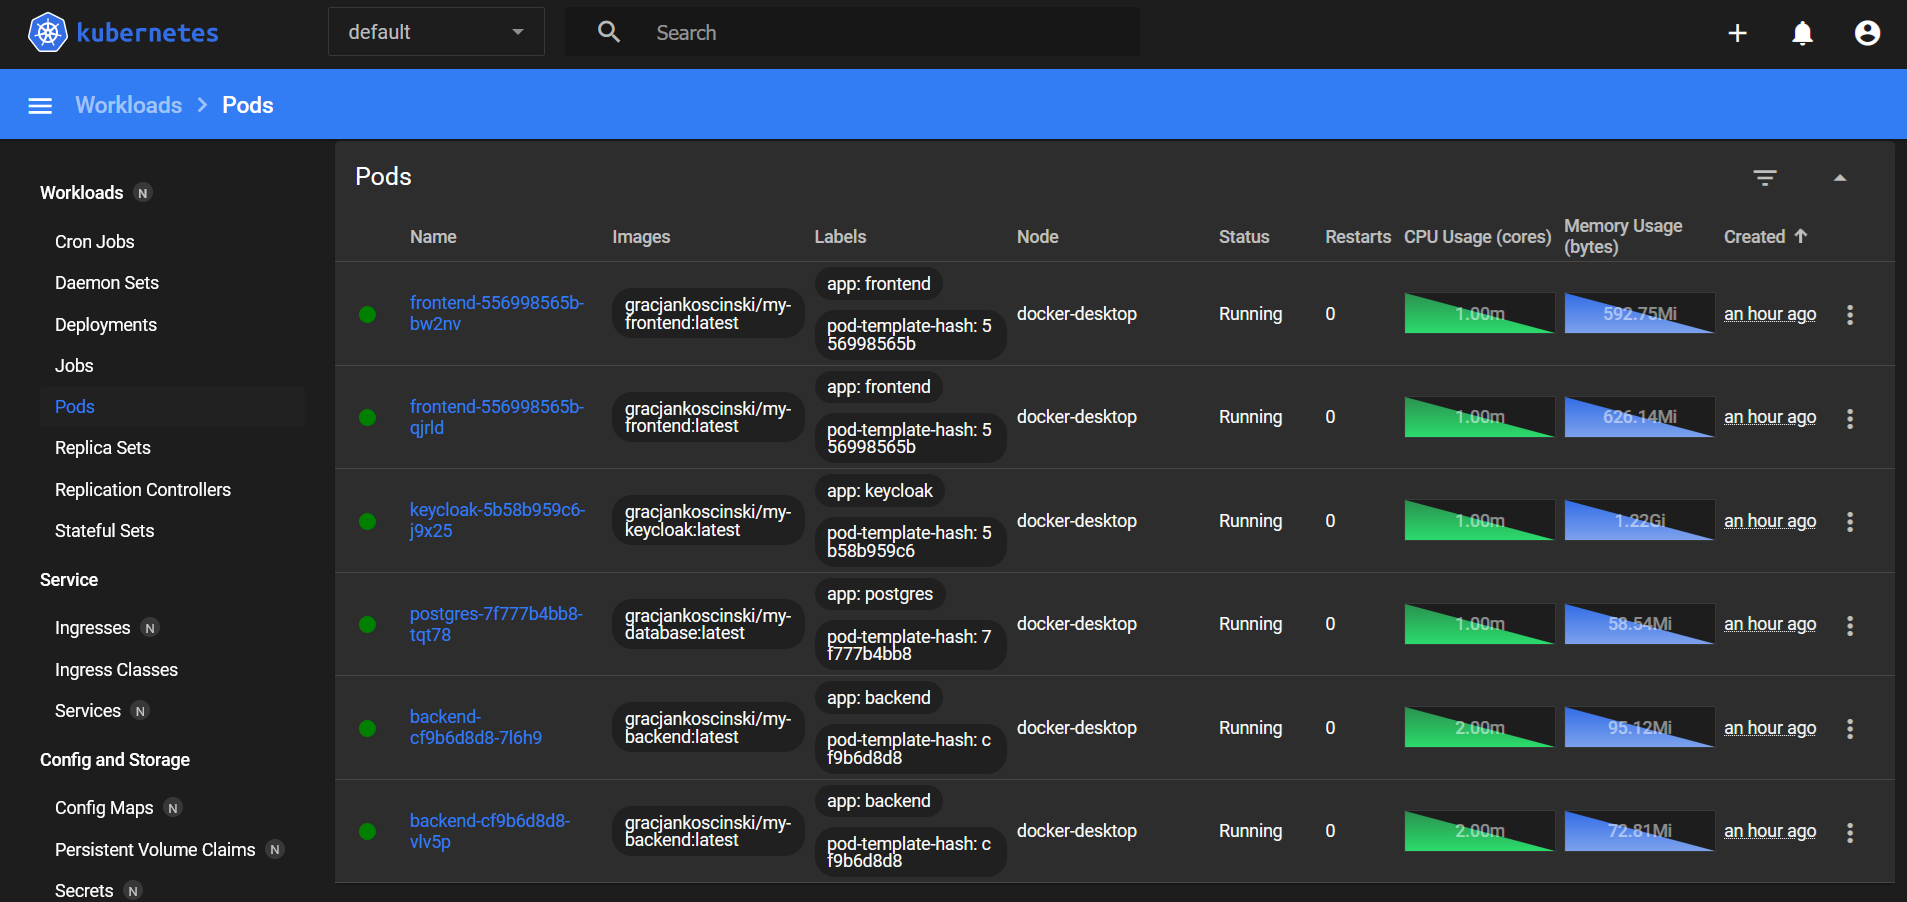
\includegraphics[width=15cm]{imagens/KubernetesUSAGE_1.png}
  \caption{Zużycie zasobów.}
\end{figure}
\begin{figure}[h]
  \centering
  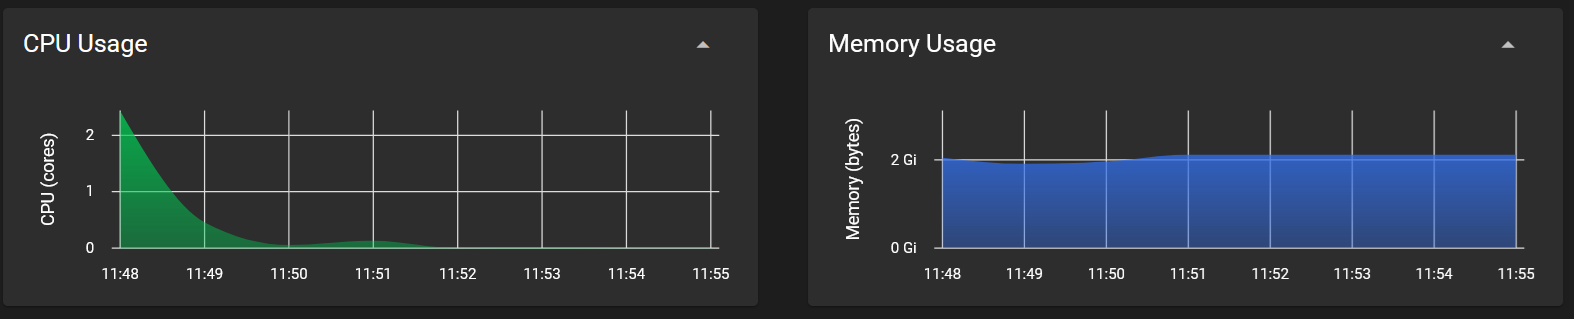
\includegraphics[width=15cm]{imagens/KubernetesUSAGE_2.png}
  \caption{Zużycie zasobów.}
\end{figure}
\subsection{Architektura sieciowa}
\label{sec:ExampleResults}

Architektura sieciowa aplikacji w kontekście środowiska opartego na Kubernetes pełni kluczową rolę w zapewnieniu prawidłowego funkcjonowania oraz bezpieczeństwa komunikacji między komponentami aplikacji oraz z zewnętrznymi użytkownikami. Zastosowanie odpowiednich mechanizmów komunikacyjnych jest niezbędne do skutecznego zarządzania ruchem sieciowym oraz zapewnienia wysokiej dostępności i wydajności systemu.
\begin{itemize}
    \item \textbf{ClusterIP Services} Usługi typu ClusterIP są używane do wewnętrznej komunikacji między różnymi komponentami aplikacji w obrębie klastra Kubernetes. Każda usługa typu ClusterIP otrzymuje wirtualny adres IP, który jest dostępny tylko w obrębie klastra. To pozwala na bezpieczną i efektywną komunikację między aplikacjami, które mogą być uruchomione na różnych węzłach w klastrze. Usługi typu ClusterIP są zazwyczaj wykorzystywane do zapewnienia komunikacji między mikroserwisami oraz komponentami wewnętrznymi aplikacji.
    \item \textbf{NodePort/LoadBalancer Services} Usługi typu NodePort umożliwiają eksponowanie aplikacji na zewnątrz klastra Kubernetes poprzez przypisanie stałego portu na każdym węźle klastra. To pozwala na dostęp do aplikacji z poziomu zewnętrznych systemów oraz urządzeń. NodePort jest używany w przypadkach, gdy aplikacja musi być dostępna z zewnątrz klastra, np. do interakcji z klientami, użytkownikami lub innymi systemami zewnętrznymi.
\end{itemize}
\bibliographystyle{amsplain}
\bibliography{references.bib}
\noindent
\nocite{*}

\end{document}